\newpage%\noindent\dotfill
\begin{multicols}{2}
\section*{Chapter Three - Rings and modules}

\begin{definition}
A \textbf{ring} is a set with two operations $(R,+,\cdot)$ such that
\begin{itemize}
    \item $(R,+)$ is an abelian group,
    \item $(R,\cdot)$ is a \textbf{monoid} (associative with identity),
    \item $\cdot$ distributes over $+$; $a\cdot(b+c)\cdot d=a\cdot b\cdot d+a\cdot c\cdot d$.
\end{itemize}
\end{definition}

\begin{definition}
A \textbf{field} is a commutative ring with inverses.
\end{definition}

\begin{theorem}[3.1.11]
The ring $\Z/m\Z$ is a field iff $m$ is prime.
\end{theorem}

\begin{definition}
An element $a\in R$ for a ring $R$ is a \textbf{unit} if it is invertible. We define $R^\times$ as the \textbf{group of units}.
\end{definition}

\begin{definition}
An element $a\in R$ for a ring $R$ is a \textbf{zero-divisor} if $\exists b\in R: b\neq0$ and $ab=0$ or $ba=0$.
\end{definition}

\begin{definition}
An \textbf{integral domain} is a non-zero commutative ring with no zero-divisors.
\end{definition}

\begin{theorem}
If $I$ is an integral domain then $ab=0\implies a=0$ or $b=0$. Moreover (3.2.16), if $ab=ac$ and $a\neq0$ then $b=c$.
\end{theorem}

\begin{theorem}]3.2.18
Every finite integral domain is a field.
\end{theorem}

\begin{definition}
The \textbf{ring of polynomials} with coefficients in a ring $R$ is denoted $R[X]$.
\end{definition}

\begin{theorem}[3.3.3]
If $R$ is a ring with no zero-divisors then $R[X]$ has no zero-divisors and $\deg(PQ)=\deg(P)+\deg(Q)$. If $R$ is an integral domain then so is $R[X]$.
\end{theorem}

\begin{theorem}[3.3.4]
Let $R$ be an integral domain with $P,Q\in R[X]$ with $Q(X)$ \textbf{monic} (leading term has coefficient one). Then $\exists! A,B\in R[X]: P=AQ+B$ with $\deg(B)<\deg(Q)$ or $B=0$.
\end{theorem}

\begin{definition}
The \textbf{evaluation} of $P\in R[X]$ at $\lambda\in R$ is $P(\lambda)$, the image of $\epsilon:R[X]\to\Maps(R,R)$. Then $\lambda$ is a \textbf{root} if $P(\lambda)=0$.
\end{definition}

\begin{theorem}[3.3.9]
Let $R$ be a commutative ring, then $\lambda\in R$ is a root of $P\in R[X]$ iff $(X-\lambda)$ divides $P(X)$.
\end{theorem}

\begin{theorem}[3.3.10]
If $P\in R[X]$ then $P$ has at most $\deg(P)$ roots in $R$.
\end{theorem}

\begin{definition}
A field is \textbf{algebraically closed} if every non-constant polynomial has a root.
\end{definition}

\begin{theorem}
The \textbf{fundamental theorem of algebra} is that $\C$ is algebraically closed.
\end{theorem}

\begin{theorem}[3.3.14]
If $F$ is an algebraically closed field then any non-zero polynomial $P(X)\in F[X]$ can be decomposed into linear factors; $P(X) = c(X-\lambda_1)\dots(X-\lambda_n)$.
\end{theorem}

\begin{definition}
Let $R$ and $S$ be rings, then $f:R\to S$ is a \textbf{ring homomorphism} if $\forall x,y\in R: f(x+y)=f(x)+f(y)$ and $f(xy)=f(x)f(y)$.
\end{definition}

\begin{theorem}[3.4.5]
Let $f\in\Hom(R,S)$ be a ring-homomorphism. Then $f(0_R)=0_S$, $f(-x)=-f(x)$ and $f(x-y)=f(x)-f(y)$.
\end{theorem}

\begin{definition}
A subset of a ring $\emptyset\neq I\subseteq R$ is an \textbf{ideal} of $R$ if $I$ is closed under subtraction and $\forall i\in I,r\in R: ir,ri\in I$. 
\end{definition}

\begin{definition}
The \textbf{ideal generated by a subset} $T\subseteq R$ is $_R\langle T\rangle := \{r_1t_1 + \dots r_nt_n : \forall i\, r_i\in R\text{ and } t_i\in T\}$. It is the \textit{smallest} ideal of $R$ that contains $T$ (prop 3.4.14).
\end{definition}

\begin{definition}
An ideal $I$ is a principle ideal if it's generated by one element, $I=\langle t\rangle$.
\end{definition}

\begin{theorem}
The \textbf{subring test} gives that $R'\subset R$ is a subring of $R$ iff
\begin{itemize}
    \item $R'$ has a multiplicative identity
    \item $R'$ is closed under subtraction
    \item $R'$ is closed under multiplication
\end{itemize}
\end{theorem}

\begin{theorem}[2.4.29]
If $f:R\to S$ is a ring homomorphism then $\text{im}(f)$ is a subring of $S$. Further, if $f(1_R)=1_S$ and $x$ is a unit in $R$ then $f(x^{-1})=f(x)^{-1}$, so $f$ restricts to the group homomorphism $f^\times: R^\times \to S^\times$.
\end{theorem}

\begin{definition}
A relation $\sim$ is an \textbf{equivalence relation} iff
\begin{itemize}
    \item $\sim$ is Reflexive; $x\sim x$
    \item $\sim$ is Symmetric; $x\sim y \implies y\sim x$
    \item $\sim$ is transitive; $(x\sim y\ and\ y\sim z)\implies x\sim z$.
\end{itemize}
\end{definition}

\begin{definition}
If $\sim$ is an equivalence relation then the \textbf{equivalence class} of $x$ is $E(x):=\{y\,:\,x\sim y\}$.
\end{definition}

\begin{definition}
The \textbf{set of equivalence classes} is $(X/\sim) \subseteq\mathcal{P}(X)$, with \textbf{canonical map} $\mathrm{can:}X\to (X/\sim),x\mapsto E(x)$.
\begin{center}
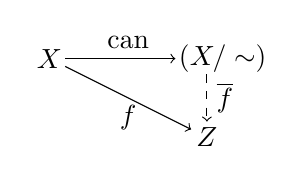
\begin{tikzpicture}
  \filldraw (0,0)node{$X$} circle (0pt);
  \filldraw (2.2,0)node{$(X/\sim)$} circle (0pt);
  \filldraw (2,-1)node{$Z$} circle (0pt);
  \draw[->] (0.2, 0) -- (1.6,0);
  \draw[->] (0.2,-0.1) -- (1.8,-0.9);
  \draw[->,dashed] (2,-0.2) -- (2,-0.8);
  \filldraw (1,0)node[anchor=south]{can} circle (0pt);
  \filldraw (2,-.5)node[anchor=west]{$\overline{f}$} circle (0pt);
  \filldraw (1,-.75)node{$f$} circle (0pt);
\end{tikzpicture}
\end{center}
A map $g:(X/\sim)\to Z$ is \textbf{well-defined} if $\exists f:X\to Z$ such that $x\sim y \implies f(x)=f(y)$ and $f$ restricts to $g$.
\end{definition}

\begin{definition}
Let $I$ be an ideal of $R$, then the \textbf{coset of $I$} is $x+I:=\{x+i\,:\,i\in I\}$.
\end{definition}

\begin{definition}
Let $I$ be an ideal of $R$ and $\sim$ be defined by $x\sim y \Leftrightarrow x-y\in I$ then $R/I=(R/\sim)$ is the \textbf{factor/quotient ring of $R$ by $I$}.
\end{definition}

\begin{theorem}
The \textbf{first isomorphism theorem} is that for rings $R,S$ we have $\forall f\in\Hom(R,S): \overline{f}:R/\ker f \tilde{to} \text{im}(f)$.
\end{theorem}

\begin{definition}
A \textbf{(left) module over R} is a pair $(M,\dot{+})$ and mapping $R\times M\to M, (r,a)\to ra$ such that for $a,b\in M$ and $r,s\in R$:
\begin{itemize}
    \item $r(a\dot{+}b) = (ra)\dot{+}(rb)$,
    \item $(r+s)a = (ra)\dot{+}(sa)$,
    \item $r(sa) = (rs)a$, and
    \item $1_Ra = a$.
\end{itemize}
\end{definition}

\begin{theorem}[3.7.8]
If $M$ is an $R$-module then $\forall a\in M: 0_Ra=0_M$, $\forall r\in R: r0_M=0_M$ and $(-r)a=r(-a)=-(ra)$.
\end{theorem}

\begin{theorem}[3.7.21]
Let $M,N$ be $R$-modules with $f\in\Hom(M,N)$, then $\ker f$ is a sub-module of $M$ and $\text{im}(f)$ is a sub-module of $N$. Moreover (3.7.22) $f$ is injective iff $\ker f = \{0_M\}$.
\end{theorem}

\begin{theorem}[3.7.29]
The intersection of any collection of sub-modules of $M$ is a sub-module of $M$.
\end{theorem}

\begin{definition}
Let $N$ be a sub-module of $M$. The set $a+N:=\{a+b\,:\,b\in N\}$ is the \textbf{coset of $M$ by $N$}, which defines the \textbf{quotient} $(M/\sim)$.
\end{definition}

\begin{theorem}
Let $R$ be a ring with $L,M$ being $R$-modules and $N\subseteq M$ a sub-module of $M$. The canonical map $\text{can}:M\to M/N$ is a surjective $R$-homomorphism with kernel $N$, and if $f(N)=\{0_L\}$ (i.e. $N\subseteq\ker f$) then $\exists!\overline{f}:M/N\to L$ such that $f=\overline{f}\circ\text{can}$.
\end{theorem}

\begin{theorem}
The \textbf{First Isomorphism Theorem}. Let $R$ be a ring with modules $M$ and $N$, then $\forall f\in\Hom(M,N)$ there is an $R$-isomorphism
    \[
    \overline{f}:M/\ker f \tilde{\to} \text{im} f.
    \]
\end{theorem}

\end{multicols}